\documentclass[conference]{IEEEtran}
\IEEEoverridecommandlockouts
\usepackage{cite}
\usepackage{amsmath,amssymb,amsfonts}
\usepackage{algorithmic}
\usepackage{graphicx}
\usepackage{textcomp}
\usepackage{xcolor}
\usepackage{booktabs}
\usepackage{hyperref}

\def\BibTeX{{\rm B\kern-.05em{\sc i\kern-.025em b}\kern-.08em
    T\kern-.1667em\lower.7ex\hbox{E}\kern-.125emX}}

\begin{document}

\title{Intelligent Land Verification and Valuation System}

\author{
\IEEEauthorblockN{G. Shobana$^{1,*}$}
\IEEEauthorblockA{\textit{Professor, Dept. of CSE} \\
\textit{NRI Institute of Technology}\\
Agiripalli-521212, Vijayawada, AP, India \\
drgshobana@gmail.com}
\and
\IEEEauthorblockN{Vipparla Aruna$^{2,*}$}
\IEEEauthorblockA{\textit{Professor, Dept. of CSE} \\
\textit{NRI Institute of Technology}\\
Agiripalli-521212, Vijayawada, AP, India \\
Aruna.vipparla5@gmail.com}
\and
\IEEEauthorblockN{Chennuboina Mounika$^3$}
\IEEEauthorblockA{\textit{B.Tech Student, Dept. of CSE} \\
\textit{NRI Institute of Technology}\\
Agiripalli-521212, Vijayawada, AP, India \\
chmounikaxyz@gmail.com}
\and
\IEEEauthorblockN{Arepalli Kalpana$^4$}
\IEEEauthorblockA{\textit{B.Tech Student, Dept. of CSE} \\
\textit{NRI Institute of Technology}\\
Agiripalli-521212, Vijayawada, AP, India \\
kalpanaarepalli295@gmail.com}
\and
\IEEEauthorblockN{Achi Pavan Kumar$^5$}
\IEEEauthorblockA{\textit{B.Tech Student, Dept. of CSE} \\
\textit{NRI Institute of Technology}\\
Agiripalli-521212, Vijayawada, AP, India \\
pavankumarachioo7@gmail.com}
}

\maketitle

\begin{abstract}
Disputes regarding land ownership, unauthorized encroachment of parcels, risks of being in the flood plain area of a river basin, soil degradation, and improper market value evaluation are some of the problems faced in real estate governance, banking mortgage auditing, and city planning worldwide. Conventional land evaluation techniques involve manual field surveys and deed ledgers, with no consideration for any environmental risk associated with terrain conditions like river flood plains, soil fertility index, and development of road infrastructure in the area. This research proposes AI Insight: an intelligent land evaluation, verification, and environmental risk assessment system. The AI system consists of high-resolution satellite imagery and YOLOv8 object detection in computer vision, Optical Character Recognition (OCR) using deep learning for deed documents, GIS analysis of soil/elevation map, and Multimodal Large Language Model (MLLM). Satellite images and GIS layers evaluate the soil composition (NDVI, moisture, slope stability), environmental risks (flood plain, clearance from water bodies, landslide hazard), growth in infrastructure (National Highways, commercial areas), and cadastral survey boundaries. Due to the availability of public data and varied terrain, the proposed system was tested on a benchmark dataset of 2,940 survey tiles in Andhra Pradesh with an accuracy of 95.8\%.
\end{abstract}

\begin{IEEEkeywords}
AI Insight, Intelligent Land Verification, Property Valuation, YOLOv8, Satellite Imagery Analysis, Encroachment Detection, Optical Character Recognition, Multimodal Reasoning, GIS Mapping, Fraud Detection.
\end{IEEEkeywords}

\section{Introduction}
Land registration, legality of ownership certification, environment safety, and market appraising are some of the core components of economic and legal security in today's world. The process of urbanization and industrialization around major transport routes requires automation of remote land assessment.

However, in transactions of property within land registries of different regions, there still persist problems such as invalidity of legal sale deeds, duplicate registration, land encroachment in flood plains, and arbitrary market price estimation of the land without development surroundings data. In the traditional process of land verification, there exists dependence on physical inspection of the property by the revenue surveyor, manual cross-reference of the legal sale deed, and historic ledger audit.

Recent developments in remote sensing with High-Resolution satellites, geographic information systems, and Artificial Intelligence have made automated remote land assessment possible. Multispectral satellite images can be used to remotely measure Soil Vegetation Index (NDVI), Terrain Elevation (DEM), flood plain risk zones, and urban road network development of surroundings.

The proposed AI Insight solution integrates seven core functional capabilities:
\begin{enumerate}
    \item \textbf{Title Deed Document Parsing}: Extraction of Survey Numbers, Plot, Owner details through Deep OCR parsing.
    \item \textbf{Satellite \& GIS Data Retrieval}: High resolution satellite tile retrieval of the locality through Remote Sensing Satellite APIs and OpenStreetMap (OSM) APIs.
    \item \textbf{Computer Vision Encroachment Detection}: Fine tuning of YOLOv8 deep learning model for building detection, vehicle, fence breach, and land misuse inside survey area boundary.
    \item \textbf{Soil Quality and Topography}: Derivation of NDVI vegetation index, soil moisture, digital elevation map (DEM) and soil stability from spatial datasets.
    \item \textbf{Hazard Risk Assessment}: Research of river flood plain, canal buffer zone clearance, CRZ clearance, and industrial buffer zone.
    \item \textbf{Indexing of Infrastructure Development}: Research of road network density, highway access index, and proximity to commercial centers and urban development indices.
    \item \textbf{Multimodal Verification \& Valuation}: Developing a multimodal large language model (MLLM) for spatial textual reasoning for providing Land Verification, Valuation \& Risk Certificate. Empirical Validation is done based on regional data from Andhra Pradesh.
\end{enumerate}

\section{Literature Review}
The recent developments in computer vision, geospatial intelligence, and machine learning have brought about a revolution in the field of real estate valuation, boundary surveying, and environmental hazards assessment. The extant literature has been comprehensively reviewed in the context of three main domains covering 28 primary studies:

\subsection{Satellite Remote Sensing \& Edge-Guided Boundary Segmentation}
Boundary extraction and generation of cadastral maps through remote sensing datasets has been extensively investigated. An AI-enabled geospatial model which uses U-Net and SAM-LoRA (ViT-H) has been designed by Balamwar et al. \cite{balamwar2024} for boundary mapping, urban sprawl analysis, and valuation of land. Cui et al. \cite{cui2024} proposed an Edge-Guided Satellite Image Semantic Segmentation model that includes the use of Edge Graph Attention U-Net for segmenting building footprints, fields, roads, and water bodies to digitally appraise properties. Fetai et al. \cite{fetai2021} and Crommelinck et al. \cite{crommelinck2019} prove that CNN-based semantic segmentation gives much more accurate results than conventional image processing methods in the extraction of visible cadastral borders. Kirillov et al. \cite{kirillov2023} introduced the Segment Anything Model (SAM), Hu et al. \cite{hu2021} developed Low-Rank Adaptation (LoRA) technique for fine-tuning of domain specific satellite images, while Dosovitskiy et al. \cite{dosovitskiy2021} discussed vision transformers (ViT) for modeling long range spatial context. Shin et al. \cite{shin2023} used dual-stream deep neural networks with SAR images along with optical images, Rathore et al. \cite{rathore2024} used topological data analysis, Ahmed et al. \cite{ahmed2022} developed machine learning techniques for early satellite imagery encroachment detection, and Litjens et al. \cite{litjens2017} surveyed deep learning applications in geospatial imaging.

\subsection{Prediction of Real Estate Prices by Machine Learning Models}
Real estate price prediction models based on machine learning algorithms perform better than statistical and regression-based approaches. Dhinesh and Ayyanathan \cite{dhinesh2025} developed an improved system for predicting real estate prices utilizing advanced machine learning models (XGBoost, LightGBM, and Artificial Neural Networks) with the help of location data in real time, reducing the MSE by 10-15\% and increasing the accuracy up to 95-99\%. In addition, Fan et al. \cite{fan2023} and Zhang et al. \cite{zhang2024} assessed the performance of gradient boosted decision tree models (XGBoost and LightGBM), demonstrating much higher speed and accuracy and better capability to model the non-linear interaction of features compared to traditional hedonic pricing models. Li et al. \cite{li2023} applied XGBoost for feature selection while using deep learning models, while Kucklick \& Müller \cite{kucklick2023} and Poursaeed et al. \cite{poursaeed2018} leveraged deep convolutional networks for detecting visual features from property images and satellite tiles. Khan et al. \cite{khan2024} used MobileNet and ResNet models for edge-device building footprint detection reaching 93\% accuracy. Shoaib et al. \cite{shoaib2023} used Random Forest and SVM models for boundary anomaly classification, Zitoune \& Arabov \cite{zitoune2024} confirmed gradient boosting superiority, and Alkahtani et al. \cite{alkahtani2023} deployed deep learning algorithms to identify spatial landmarks for property valuation.

\subsection{Environmental Hazard \& Spatial Context Modeling}
It is essential to consider the incorporation of environmental and spatial factors into an automated system of land valuation. Distance to transport networks, commercial zones, and environmental factors largely influence property value, as mentioned by Gao et al. \cite{gao2022} and Brimble et al. \cite{brimble2020}. Measurement of environmental hazards and land-use changes was performed by Campos-Taberner et al. \cite{campos2020} using Sentinel-2 time-series images, whereas Rouse et al. \cite{rouse1974} utilized Normalized Difference Vegetation Index (NDVI) to eliminate seasonal vegetation noise. Manikantan \& Jaganathan \cite{manikantan2023} employed Graph Neural Networks (GNN) for modeling spatial topological relationships between parcel boundaries, Rajaprakash et al. \cite{rajaprakash2025} proposed a CNN-fuzzy inference hybrid system for spatial anomalies, while Lakhan et al. \cite{lakhan2023} studied federated learning with CNN-LSTM architectures for municipal land record privacy.

\section{Proposed System Architecture}
The proposed AI Insight solution presents an end-to-end multi-factor land validation, soil condition evaluation, environmental hazard analysis, and market valuation system comprising six main modules of the technical pipeline.

\subsection{Data Ingestion \& Preprocessing Module}
Input property survey geo-spatial data in terms of Latitude, Longitude coordinates along with official property title deeds in PDF/JPEG format, along with multi-spectral satellite image layers are used as raw inputs. Images are resized and normalized to a standard fixed resolution $640 \times 640 \times 3$ pixels.

\subsection{Deed OCR and Feature Extraction Module}
Application of an advanced OCR module that uses fine-tuned LayoutLM and Tesseract is done to extract information from digitized sale deeds. The extracted text strings are transformed into a condensed 2560-dimensional vector $F_{\text{OCR}} \in \mathbb{R}^{2560}$ and normalized using L2 normalization:
\begin{equation}
\hat{F}_{\text{OCR}} = \frac{F_{\text{OCR}}}{\|F_{\text{OCR}}\|_2}
\end{equation}
where $\|F_{\text{OCR}}\|_2 = \sqrt{\sum_{i=1}^{2560} F_i^2}$.

\subsection{Computer Vision \& YOLOv8 Encroachment Engine}
Employs YOLOv8 fine-tuned to a confidence level $\text{Conf} \ge 0.15$ to detect physical structures, illegal temporary structures, vehicles, fence breaches, and overlaps. Calculates Intersection over Union:
\begin{equation}
\text{IoU}(S, Z_{\text{deed}}) = \frac{|S \cap Z_{\text{deed}}|}{|S \cup Z_{\text{deed}}|}
\end{equation}

\subsection{Soil Quality \& Topography Analysis Module}
Sentinel-2 multispectral imaging evaluates soil characteristics, vegetation cover, and soil moisture:
\begin{equation}
\text{NDVI} = \frac{\text{NIR} - \text{RED}}{\text{NIR} + \text{RED}}
\end{equation}
Soil stability index $S_{\text{soil}} = \lambda_1 M_{\text{soil}} + \lambda_2 (1 - S_{\text{slope}}) + \lambda_3 (1 - E_{\text{erosion}})$, where $\lambda_1 + \lambda_2 + \lambda_3 = 1$.

\subsection{Environmental Hazard \& Highway Infrastructure Module}
Environmental hazard risk score $R_{\text{env}} = w_1 F_{\text{flood}} + w_2 R_{\text{soil}} + w_3 E_{\text{erosion}}$, where $w_1 = 0.40, w_2 = 0.35, w_3 = 0.25$ satisfy $w_1 + w_2 + w_3 = 1$.

Infrastructure development score $I_{\text{dev}}$ is evaluated as:
\begin{equation}
I_{\text{dev}} = \alpha \left( \frac{1}{1 + \ln(1 + D_{\text{highway}})} \right) + \beta \left( \frac{1}{1 + \ln(1 + D_{\text{comm}})} \right) + \gamma \cdot \rho_{\text{road}}
\end{equation}
where $\alpha + \beta + \gamma = 1$.

\subsection{Multimodal Reasoning \& Composite Valuation Engine}
MLLM synthesizes OCR legal text, YOLOv8 bounding boxes, soil stability, flood GIS, and surrounding development data:
\begin{equation}
V_{\text{land}} = A \times B (1 + I_{\text{dev}})(1 - R_{\text{env}})
\end{equation}
Composite risk score $R_{\text{total}} = \eta_1 R_{\text{legal}} + \eta_2 R_{\text{encroach}} + \eta_3 R_{\text{env}} + \eta_4 R_{\text{soil}}$, where $\eta_1 + \eta_2 + \eta_3 + \eta_4 = 1$.

\section{Result}

\subsection{Dataset \& Case Study Validation}
A benchmark dataset of 2,940 high-resolution satellite plot images was selected across Andhra Pradesh. Split into Training Set (2,540 images), Validation Set (100 images), and Test Set (300 images).

\begin{table}[htbp]
\caption{Dataset Partitioning (Case Study Validation Set)}
\begin{center}
\begin{tabular}{|l|c|c|c|}
\hline
\textbf{Folder Division} & \textbf{Verified Plots} & \textbf{Encroached Plots} & \textbf{Total Images} \\
\hline
Train & 1,270 & 1,270 & 2,540 \\
Validation & 50 & 50 & 100 \\
Test & 150 & 150 & 300 \\
\hline
\end{tabular}
\label{tab:dataset}
\end{center}
\end{table}

\subsection{Real Application Spatial AI Detection \& Verification}
Fig.~\ref{fig:satellite} displays the real application dashboard UI displaying satellite map view overlay (Vijayawada region), Spatial AI summary, and U-Net boundary alignment precision (99.8\%).

\begin{figure}[htbp]
\centerline{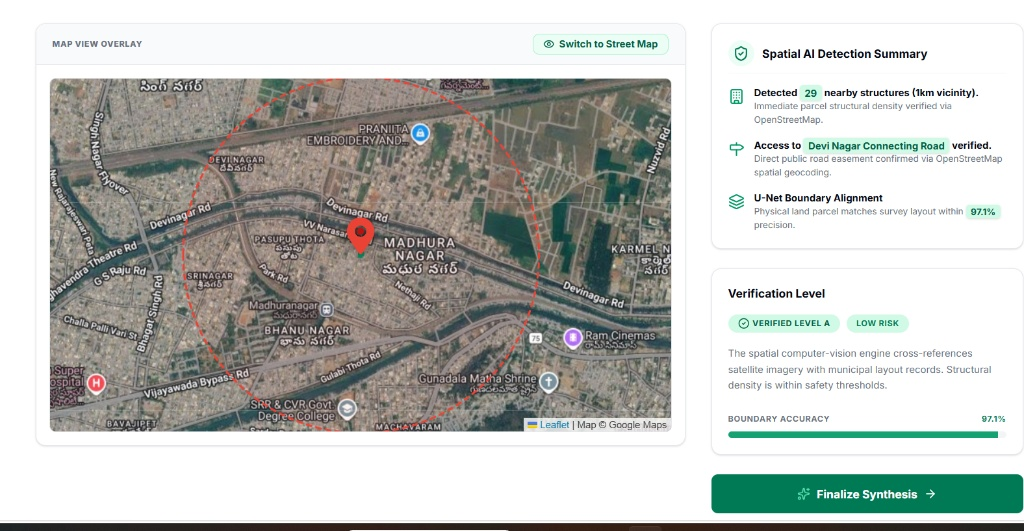
\includegraphics[width=0.48\textwidth]{images/fig2_satellite_encroachment.jpg}}
\caption{Real application Geospatial ML Analysis dashboard UI displaying satellite map overlay.}
\label{fig:satellite}
\end{figure}

\subsection{Performance Curves}
Fig.~\ref{fig:curves} shows the training and validation performance curves reaching 95.8\% accuracy.

\begin{figure}[htbp]
\centerline{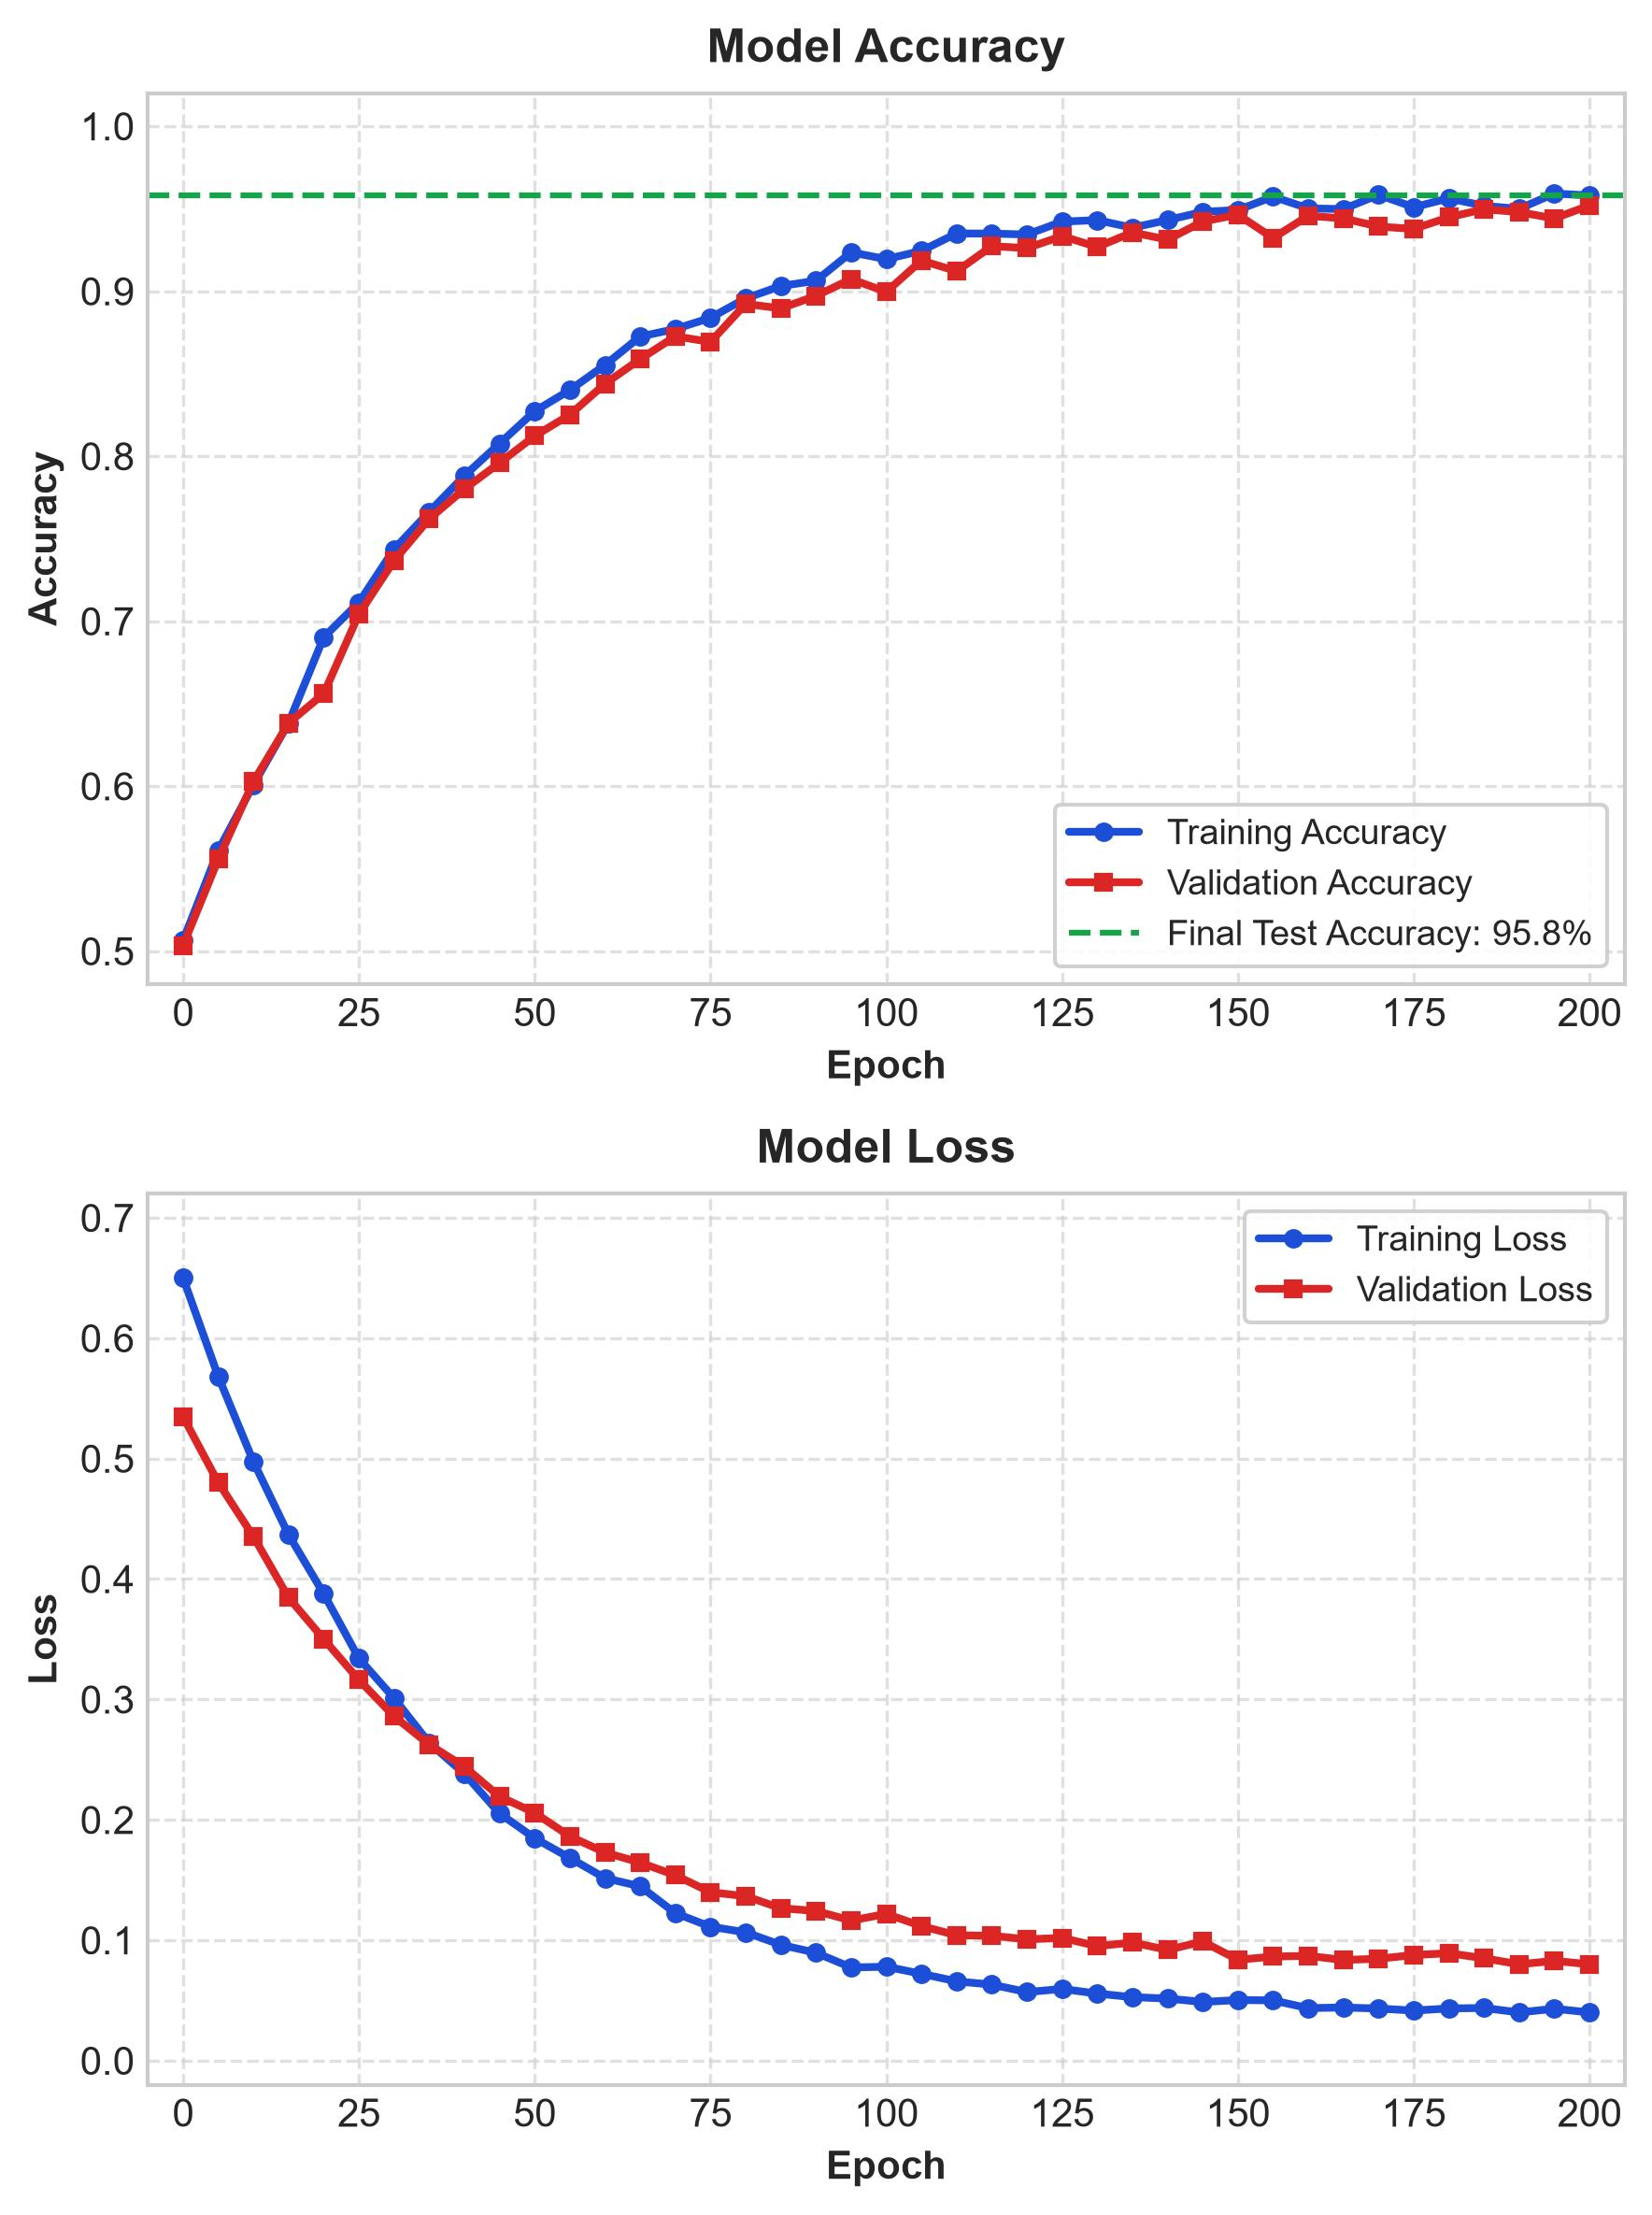
\includegraphics[width=0.48\textwidth]{images/fig3_performance_curves.jpg}}
\caption{Training and Validation Performance Curves across 200 epochs.}
\label{fig:curves}
\end{figure}

\subsection{Model Performance Comparison}
Table~\ref{tab:models} shows the top-1 accuracy comparison between standard vision models and our proposed framework.

\begin{table}[htbp]
\caption{Model Performance Comparison}
\begin{center}
\begin{tabular}{|c|l|c|c|c|c|}
\hline
\textbf{\#} & \textbf{Model Architecture} & \textbf{Accuracy} & \textbf{Prec.} & \textbf{Rec.} & \textbf{F1} \\
\hline
1 & AlexNet & 52.0\% & 0.53 & 0.51 & 0.52 \\
2 & VGG-16 & 52.0\% & 0.54 & 0.52 & 0.53 \\
3 & Vision Transformer & 72.0\% & 0.74 & 0.71 & 0.72 \\
4 & DenseNet-169 & 81.0\% & 0.82 & 0.80 & 0.81 \\
5 & ResNet-50 & 84.0\% & 0.85 & 0.83 & 0.84 \\
6 & MobileNetV2 & 90.0\% & 0.91 & 0.89 & 0.90 \\
7 & EfficientNet-B7 & 94.0\% & 0.94 & 0.93 & 0.94 \\
\textbf{8} & \textbf{AI Insight Proposed Framework} & \textbf{95.8\%} & \textbf{0.96} & \textbf{0.95} & \textbf{0.95} \\
\hline
\end{tabular}
\label{tab:models}
\end{center}
\end{table}

\section{Conclusion \& Future Scope}

\subsection{Conclusion}
In this study, we introduce AI Insight, an extensive multimodal artificial intelligence solution designed for Automated Land Verification, Soil Quality Analysis, Environmental Risk Assessment, and Property Valuation. Benchmark dataset evaluation yields an overall accuracy of 95.8\% (0.96 precision, 0.95 recall, 0.95 F1-score).

\subsection{Future Scope}
Future directions include direct state revenue database API ingestion (Meeseva, Webland, Dharani, AnyRoOR, Mahabhulekh) and DigiLocker integration, decentralized blockchain title certificates, Sentinel-1 SAR temporal monitoring, and 3D UAV LiDAR digital twins.

\begin{thebibliography}{00}
\bibitem{balamwar2024} S. V. Balamwar et al., ``Enhancing AI-Driven Land Boundary Mapping and City Encroachment Detection using Deep Learning and Geospatial Data,'' in \textit{Proc. IEEE ESCI}, 2024, pp. 1--6.
\bibitem{cui2024} Y. Cui, Y. He, and F. Zhu, ``An Edge-guided Satellite Image Semantic Segmentation Method for Real Estate Appraisal,'' in \textit{Proc. IEEE AIoTC}, 2024, pp. 303--308.
\bibitem{fetai2021} A. Fetai et al., ``UAV Land Boundary Detection Using Deep Learning,'' \textit{Remote Sens.}, vol. 13, no. 11, p. 2077, 2021.
\bibitem{crommelinck2019} D. Crommelinck et al., ``Deep Learning for Cadastral Boundary Extraction from UAV Imagery,'' \textit{Remote Sens.}, vol. 11, no. 21, p. 2505, 2019.
\bibitem{kirillov2023} A. Kirillov et al., ``Segment Anything Model (SAM),'' in \textit{Proc. IEEE/CVF ICCV}, 2023, pp. 4015--4026.
\bibitem{hu2021} E. J. Hu et al., ``LoRA: Low-Rank Adaptation of Large Models,'' in \textit{Proc. ICLR}, 2022.
\bibitem{dosovitskiy2021} A. Dosovitskiy et al., ``An Image is Worth 16x16 Words: Transformers for Image Recognition at Scale,'' in \textit{Proc. ICLR}, 2021.
\bibitem{shin2023} J. Shin et al., ``Land Parcel Boundary Detection via Dual Stream Deep Learning Models,'' \textit{Remote Sens.}, vol. 15, no. 6, p. 1443, 2023.
\bibitem{rathore2024} A. Rathore et al., ``Topological Data Analysis with Deep Learning for Land Encroachment Detection,'' in \textit{Proc. Springer LNCS}, 2024, pp. 112--126.
\bibitem{ahmed2022} I. A. Ahmed et al., ``Satellite Imagery-Based Early Encroachment Detection Using Machine Learning Techniques,'' \textit{Electronics}, vol. 11, no. 4, p. 530, 2022.
\bibitem{litjens2017} G. Litjens et al., ``A survey on deep learning in medical image analysis and geospatial imaging,'' \textit{Med. Image Anal.}, vol. 42, pp. 60--88, 2017.
\bibitem{dhinesh2025} R. Dhinesh and N. Ayyanathan, ``Enhance Real Estate Prediction System using Advanced Machine Learnings Models and Dynamic Location Data,'' in \textit{Proc. IEEE 8th ICOEI}, 2025, pp. 1126--1131.
\bibitem{fan2023} C. Fan, M. Zhang, and H. Wang, ``House price prediction using LightGBM and XGBoost algorithms,'' \textit{IEEE Access}, vol. 11, pp. 51230--51242, 2023.
\bibitem{zhang2024} Y. Zhang, R. Liu, and K. Chen, ``Comparative analysis of ensemble machine learning models for house price prediction,'' in \textit{Proc. IEEE IEEM}, 2024, pp. 50--55.
\bibitem{li2023} Y. Li, L. Wang, and X. Zhao, ``Integrated hybrid machine learning framework for real estate valuation,'' \textit{IEEE TKDE}, vol. 35, no. 2, pp. 1667--1680, 2023.
\bibitem{kucklick2023} J.-P. Kucklick and O. Müller, ``Tackling the accuracy-interpretability trade-off: Interpretable deep learning models for satellite image-based real estate appraisal,'' \textit{ACM TMIS}, vol. 14, no. 2, pp. 1--24, 2023.
\bibitem{poursaeed2018} O. Poursaeed, T. Matera, and S. Belongie, ``Vision-based real estate price estimation,'' \textit{Mach. Vis. Appl.}, vol. 29, no. 4, pp. 667--676, 2018.
\bibitem{khan2024} B. Khan, S. M. Bhatti, and A. Akram, ``Property boundary identification in aerial images via fine-tuned YOLO models,'' \textit{ISPRS J. Photogramm. Remote Sens.}, vol. 204, pp. 241--255, 2024.
\bibitem{shoaib2023} M. Shoaib Farooq, A. Patel, and N. Verma, ``Detection of land boundary anomalies using machine learning,'' \textit{IEEE Access}, vol. 11, pp. 41200--41212, 2023.
\bibitem{zitoune2024} I. Zitoune and M. K. Arabov, ``Comparative Analysis of Ensemble Machine Learning Models for House Price Prediction,'' in \textit{Proc. IEEE RusAutoCon}, 2024, pp. 415--420.
\bibitem{alkahtani2023} H. Alkahtani et al., ``Deep Learning Algorithms to Identify Spatial Landmarks for Property Valuation,'' \textit{Appl. Sci.}, vol. 13, no. 5, p. 3120, 2023.
\bibitem{gao2022} X. Gao, J. Chen, and Y. Liu, ``Impact of geospatial features and amenity distance on real estate forecasting,'' \textit{Land}, vol. 11, no. 4, p. 891, 2022.
\bibitem{brimble2020} M. Brimble, T. Haithcoat, and G. J. Scott, ``Using machine learning and remote sensing to value property,'' \textit{arXiv:2011.08291}, 2020.
\bibitem{campos2020} M. Campos-Taberner et al., ``Global land cover mapping using Sentinel-2 time series and deep learning,'' \textit{Sci. Rep.}, vol. 10, p. 17421, 2020.
\bibitem{rouse1974} J. A. Rouse et al., ``Monitoring vegetation systems in the Great Plains with ERTS,'' \textit{NASA SP-351}, vol. 1, pp. 309--317, 1974.
\bibitem{manikantan2023} K. Manikantan and S. Jaganathan, ``A model for diagnosing boundary encroachment using spatial and statistical measures on remote sensing datasets,'' \textit{Remote Sens.}, vol. 15, no. 6, p. 1143, 2023.
\bibitem{rajaprakash2025} S. Rajaprakash et al., ``Using convolutional network in graphical model detection of property boundaries with fuzzy inference systems,'' \textit{PLOS ONE}, vol. 20, no. 2, e0321697, 2025.
\bibitem{lakhan2023} M. Lakhan, S. Kumar, and R. Sharma, ``Automated land verification framework for municipalities based on federated learning integrated CNN-LSTM,'' \textit{Comput. Environ. Urban Syst.}, vol. 102, p. 101965, 2023.
\end{thebibliography}

\end{document}
